\part{实例操作}

\section{实例1:全球模拟}

本实例配置了一个常用的全球模拟的情景。实例使用了0.5\textdegree 的经纬度网格,植物群落(PC)方案的植被结构次网格,以及van Genuchten-Mualem土壤水特征曲线模型。

\texttt{define.h}文件的内容为,
\lstinputlisting[language=fortran, basicstyle=\linespread{1.0}\footnotesize\ttfamily, commentstyle=\color{olive}, numbers=left, numberstyle=\tiny, xleftmargin=1.5em,xrightmargin=0em, aboveskip=1em]{examples/global/define.h}

Namelist文件的内容为,
\lstinputlisting[language=fortran, basicstyle=\linespread{1.0}\footnotesize\ttfamily, commentstyle=\color{olive}, numbers=left, numberstyle=\tiny, xleftmargin=1.5em,xrightmargin=0em, aboveskip=1em]{examples/global/Global_Grid_50km_PC_VG.nml}

此实例中,\par
1)\textbf{并行化}方面,将全球分为20\textdegree$\times$20\textdegree 的数据块进行并行模拟(\texttt{DEF\_nx\_blocks}和\texttt{DEF\_ny\_blocks}),每24个进程为一个工作组(\texttt{DEF\_PIO\_groupsize});\par
2)\textbf{地表覆盖类型数据}使用了2005年的数据(\texttt{DEF\_LC\_YEAR});\par
3)\textbf{叶面积指数数据}使用了2005年的月数据(不随年份变化时,叶面积指数数据的年份同\texttt{DEF\_LC\_YEAR}),不随年份变化(\texttt{DEF\_LAI\_CHANGE\_YEARLY});\par
4)使用FIT算法进行\textbf{土壤水热参数升尺度}(\texttt{DEF\_USE\_SOILPAR\_UPS\_FIT});\par
5)使用冷启动的方式对土壤和积雪的状态进行\textbf{初始化}(\texttt{DEF\_USE\_SoilInit}和\texttt{\allowbreak DEF\_\allowbreak USE\_SnowInit});\par
6)对以下\textbf{过程参数化方案}进行了设置:
\begin{itemize}[nosep,leftmargin=4em]
    \item 降水截留(\texttt{DEF\_Interception\_scheme});
    \item 土壤热力参数(\texttt{DEF\_THERMAL\_CONDUCTIVITY\_SCHEME});
    \item 土壤阻抗(\texttt{DEF\_RSS\_SCHEME});
    \item 土壤水运动数值方案(\texttt{DEF\_USE\_VariablySaturatedFlow});
    \item 过冷水方案(\texttt{DEF\_USE\_SUPERCOOL\_WATER});
    \item 产流参数化方案(\texttt{DEF\_Runoff\_SCHEME});
    \item SNICAR模块(\texttt{DEF\_USE\_SNICAR});
    \item 雨雪拆分方案(\texttt{DEF\_precip\_phase\_discrimination\_scheme});
    \item 植被水力过程方案(\texttt{DEF\_USE\_PLANTHYDRAULICS});
    \item 气孔水利用效率方案(\texttt{DEF\_USE\_WUEST});
    \item 水体深度动态变化方案(\texttt{DEF\_USE\_Dynamic\_Lake}).
\end{itemize}
\par
7)使用CRUJRA数据作为\textbf{大气驱动}(\texttt{DEF\_forcing\_namelist});\par
8)每月保存一次\textbf{重启动}变量(\texttt{DEF\_WRST\_FREQ});\par
9)\textbf{历史数据的输出},
\begin{itemize}[nosep,leftmargin=4em]
    \item 输出到0.5\textdegree 经纬度网格(\texttt{DEF\_hist\_lon\_res}和\texttt{DEF\_hist\_lon\_res});
    \item 输出变量的月值(\texttt{DEF\_HIST\_FREQ});
    \item 每年的数据保存在一个文件中(\texttt{DEF\_HIST\_groupby});
    \item 输出所有变量(\texttt{DEF\_hist\_vars\_out\_default}).
\end{itemize}\par
10)其他配置使用模式默认值。

\section{实例2:自然植被下垫面单点模拟}

本节配置了一个仅使用CoLM自带地表数据集即可运行的单点模拟实例。实例使用地表覆盖类型(IGBP)植被结构次网格,以及van Genuchten-Mualem土壤水特征曲线模型,实时输出调试信息及检查变量范围。在单点模式下,自动关闭并行功能。

\texttt{define.h}文件的内容为,
\lstinputlisting[language=fortran, basicstyle=\linespread{1.0}\footnotesize\ttfamily, commentstyle=\color{olive}, numbers=left, numberstyle=\tiny, xleftmargin=1.5em,xrightmargin=0em, aboveskip=1em]{examples/site_soil/define.h}

Namelist文件的内容为,
\lstinputlisting[language=fortran, basicstyle=\linespread{1.0}\footnotesize\ttfamily, commentstyle=\color{olive}, numbers=left, numberstyle=\tiny, xleftmargin=1.5em,xrightmargin=0em, aboveskip=1em]{examples/site_soil/SiteSYSUAtmos_IGBP_VG.nml}

此实例中,\par
1)模拟点的地表覆盖类型、树高、叶面积指数、土壤反照率、土壤水热参数和地形等主要地表参数均根据模拟点的经纬度(\texttt{SITE\_lon\_location}和\texttt{SITE\_lat\_location})\textbf{从CoLM自带的地表数据集中提取};\par
2)模拟时间为1951年至2020年,其中2000年前为预热,预热阶段重复两次;\par
3)使用了逐年变化(\texttt{DEF\_LAI\_CHANGE\_YEARLY})\textbf{叶面积指数月数据}\\ (\texttt{DEF\_LAI\_MONTHLY});\par
4)从ERA5LAND驱动数据集中提取模拟点的\textbf{大气驱动数据};\par
5)每月保存一次\textbf{重启动}变量(\texttt{DEF\_WRST\_FREQ});\par
6)\textbf{历史数据的输出},
\begin{itemize}[nosep,leftmargin=4em]
    \item 输出变量的日值(\texttt{DEF\_HIST\_FREQ});
    \item 每年的数据保存在一个文件中(\texttt{DEF\_HIST\_groupby});
    \item 输出所有变量(\texttt{DEF\_hist\_vars\_out\_default}).
\end{itemize} \par
7)其余配置使用模式默认值。

\section{实例3:城市单点模拟}

本节配置了一个城市单点模拟实例。实例的地表覆盖类型为城市,使用CoLM 2024版新加入的城市模块,使用Campbell土壤水特征曲线模型,实时输出调试信息及检查变量范围。在单点模式下,自动关闭并行功能。

\texttt{define.h}文件的内容为,
\lstinputlisting[language=fortran, basicstyle=\linespread{1.0}\footnotesize\ttfamily, commentstyle=\color{olive}, numbers=left, numberstyle=\tiny, xleftmargin=1.5em,xrightmargin=0em, aboveskip=1em]{examples/site_urban/define.h}

Namelist文件的内容为,
\lstinputlisting[language=fortran, basicstyle=\linespread{1.0}\footnotesize\ttfamily, commentstyle=\color{olive}, numbers=left, numberstyle=\tiny, xleftmargin=1.5em,xrightmargin=0em, aboveskip=1em]{examples/site_urban/Site_AU-Preston.nml}

此实例中,\par
1)模拟点的叶面积指数、土壤反照率和土壤水热参数等地表参数根据模拟点的经纬度(从\texttt{\$SITE\_fsitedata}中读取)\textbf{从CoLM自带的地表数据集中提取};\par
2)模拟点的城市参数来源于数据文件\texttt{\$SITE\_fsitedata};\par
3)模拟时间为1993年至2004年,其中2003年8月12日前为预热;\par
4)对以下\textbf{城市参数化方案}进行了设置:
\begin{itemize}[nosep,leftmargin=4em]
    \item 模拟城市中的植被(\texttt{DEF\_URBAN\_TREE});
    \item 模拟城市中的水体(\texttt{DEF\_URBAN\_WATER});
    \item 模拟城市中的建筑能耗排放(\texttt{DEF\_URBAN\_BEM});
    \item 模拟城市中的交通热以及人体代谢热(\texttt{DEF\_URBAN\_LUCY});
    \item 使用三维建筑高边长比参数(\texttt{DEF\_USE\_CANYON\_HWR});
\end{itemize} \par
5)使用了逐年变化(\texttt{DEF\_LAI\_CHANGE\_YEARLY})\textbf{叶面积指数月数据};\par
6)对以下\textbf{过程参数化方案}进行了设置:
\begin{itemize}[nosep,leftmargin=4em]
    \item 降水截留(\texttt{DEF\_Interception\_scheme});
    \item 过冷水方案(\texttt{DEF\_USE\_SUPERCOOL\_WATER});
    \item 土壤水运动数值方案(\texttt{DEF\_USE\_VariablySaturatedFlow});
    \item 植被水力过程方案(\texttt{DEF\_USE\_PLANTHYDRAULICS});
    \item 气孔水利用效率方案(\texttt{DEF\_USE\_WUEST});
    \item SNICAR模块(\texttt{DEF\_USE\_SNICAR});
    \item 是否将土壤和积雪表面的热力过程分开计算(\texttt{DEF\_SPLIT\_SOILSNOW});
\end{itemize}
\par
7)使用模拟点观测的的\textbf{大气驱动数据}(通过\texttt{DEF\_forcing\_namelist}设置);\par
8)每月保存一次\textbf{重启动}变量(\texttt{DEF\_WRST\_FREQ}),不对重启动文件进行压缩(\texttt{DEF\_\allowbreak REST\_\allowbreak CompressLevel});\par
9)\textbf{历史数据的输出},
\begin{itemize}[nosep,leftmargin=4em]
    \item 输出每个步长的变量值(\texttt{DEF\_HIST\_FREQ});
    \item 每月的数据保存在一个文件中(\texttt{DEF\_HIST\_groupby});
    \item 不对重启动文件进行压缩(\texttt{DEF\_HIST\_CompressLevel})
    \item 输出所有变量(\texttt{DEF\_hist\_vars\_out\_default}).
\end{itemize} \par
10)其余配置使用模式默认值。

\section{实例4:生物地球化学过程模拟}

本实例配置了一个常用的全球模拟的情景。实例使用了2.5\textdegree $\times$ 1.875\textdegree 的经纬度网格,植物功能类型(PFT)方案的植被结构次网格,以及van Genuchten-Mualem土壤水特征曲线模型,打开了CoLM 2024版中新建立的生物地球化学循环过程模块。

\texttt{define.h}文件的内容为,
\lstinputlisting[language=fortran, basicstyle=\linespread{1.0}\footnotesize\ttfamily, commentstyle=\color{olive}, numbers=left, numberstyle=\tiny, xleftmargin=1.5em,xrightmargin=0em, aboveskip=1em]{examples/bgc/define.h}

Namelist文件的内容为,
\lstinputlisting[language=fortran, basicstyle=\linespread{1.0}\footnotesize\ttfamily, commentstyle=\color{olive}, numbers=left, numberstyle=\tiny, xleftmargin=1.5em,xrightmargin=0em, aboveskip=1em]{examples/bgc/Global_Grid_2x2_PFT_VG_BGC.nml}

此实例中,\par
1)\textbf{并行化}方面,将全球分为20\textdegree$\times$20\textdegree 的数据块进行并行模拟(\texttt{DEF\_nx\_blocks}和\texttt{DEF\_ny\_blocks}),每24个进程为一个工作组(\texttt{DEF\_PIO\_groupsize});\par
2)\textbf{地表覆盖类型数据}使用了2005年的数据(\texttt{DEF\_LC\_YEAR});\par
3)\textbf{叶面积指数数据}使用了2005年的月数据(不随年份变化时,叶面积指数数据的年份同\texttt{DEF\_LC\_YEAR}),不随年份变化(\texttt{DEF\_LAI\_CHANGE\_YEARLY});\par
4)使用FIT算法进行\textbf{土壤水热参数升尺度}(\texttt{DEF\_USE\_SOILPAR\_UPS\_FIT});\par
5)使用冷启动的方式对土壤和积雪的状态进行\textbf{初始化}(\texttt{DEF\_USE\_SoilInit}和\texttt{DEF\_\allowbreak USE\_\allowbreak SnowInit});\par
6)使用热启动的方式对碳和氮的状态进行\textbf{初始化}(\texttt{DEF\_USE\_CN\_Init});\par
7)对以下\textbf{过程参数化方案}进行了设置:
\begin{itemize}[nosep,leftmargin=4em]
    \item 降水截留(\texttt{DEF\_Interception\_scheme});
    \item 土壤热力参数(\texttt{DEF\_THERMAL\_CONDUCTIVITY\_SCHEME});
    \item 土壤阻抗(\texttt{DEF\_RSS\_SCHEME});
    \item 土壤水运动数值方案(\texttt{DEF\_USE\_VariablySaturatedFlow});
    \item 过冷水方案(\texttt{DEF\_USE\_SUPERCOOL\_WATER});
    \item 产流参数化方案(\texttt{DEF\_Runoff\_SCHEME});
    \item SNICAR模块(\texttt{DEF\_USE\_SNICAR});
    \item 雨雪拆分方案(\texttt{DEF\_precip\_phase\_discrimination\_scheme});
    \item 植被水力过程方案(\texttt{DEF\_USE\_PLANTHYDRAULICS});
    \item 气孔水利用效率方案(\texttt{DEF\_USE\_WUEST});
    \item 水体深度动态变化方案(\texttt{DEF\_USE\_Dynamic\_Lake}).
\end{itemize}
\par
8)使用CRUJRA数据作为\textbf{大气驱动}(\texttt{DEF\_forcing\_namelist});\par
9)每月保存一次\textbf{重启动}变量(\texttt{DEF\_WRST\_FREQ});\par
10)\textbf{历史数据的输出},
\begin{itemize}[nosep,leftmargin=4em]
    \item 输出到2.5\textdegree $\times$ 1.875\textdegree 经纬度网格(\texttt{DEF\_hist\_lon\_res}和\texttt{DEF\_hist\_lon\_res});
    \item 输出变量的月值(\texttt{DEF\_HIST\_FREQ});
    \item 每年的数据保存在一个文件中(\texttt{DEF\_HIST\_groupby});
    \item 输出所有变量(\texttt{DEF\_hist\_vars\_out\_default}).
\end{itemize}\par
11)其他配置使用模式默认值。

\section{实例5:区域高分辨率模拟}

本实例配置了一个区域高分辨率模拟情景。实例使用了1千米的经纬度网格,地表覆盖类型(IGBP)植被结构次网格,以及van Genuchten-Mualem土壤水特征曲线模型,并使用MPI进行并行加速。

\texttt{define.h}文件的内容为,
\lstinputlisting[language=fortran, basicstyle=\linespread{1.0}\footnotesize\ttfamily, commentstyle=\color{olive}, numbers=left, numberstyle=\tiny, xleftmargin=1.5em,xrightmargin=0em, aboveskip=1em]{examples/hires/define.h}

Namelist文件的内容为,
\lstinputlisting[language=fortran, basicstyle=\linespread{1.0}\footnotesize\ttfamily, commentstyle=\color{olive}, numbers=left, numberstyle=\tiny, xleftmargin=1.5em,xrightmargin=0em, aboveskip=1em]{examples/hires/GreaterBay_Grid_1km_IGBP_VG.nml}

此实例中,\par
1)区域大致范围通过\texttt{DEF\_domain}进行设定,并使用文件\texttt{DEF\_file\_mesh\_filter}中的'mesh\_filter'变量进一步细化需要模拟的\textbf{区域范围};\par
2)\textbf{并行化}方面,将全球分为180\textdegree$\times$90\textdegree 的数据块进行并行模拟(\texttt{DEF\_nx\_blocks}和\texttt{DEF\_ny\_blocks}),每24个进程为一个工作组(\texttt{DEF\_PIO\_groupsize});\par
3)使用热启动的方式对土壤状态进行\textbf{初始化}(\texttt{DEF\_USE\_SoilInit}),初始状态从文件\texttt{DEF\_file\_SoilInit}中读入;\par
4)\textbf{过程参数化方案}均使用模式默认值;\par
5)使用ERA5数据作为\textbf{大气驱动}(\texttt{DEF\_forcing\_namelist});\par
6)从粗分辨率的驱动数据到细分辨率的陆表单元使用\textbf{双线性插值}的方法\\ (\texttt{DEF\_Forcing\_Interp\_Method}),在插值的过程中同时进行\textbf{降尺度}\\ (\texttt{DEF\_USE\_Forcing\_Downscaling});\par
7)\textbf{降尺度方法}中,对降水的调整使用Liston and Elder~(2006)提出的方案\\ (\texttt{DEF\_DS\_precipitation\_adjust\_scheme}),对下行长波辐射的调整使用van Tricht et al. (2016)提出的方案(\texttt{DEF\_DS\_longwave\_adjust\_scheme});\par
8)每月保存一次\textbf{重启动}变量(\texttt{DEF\_WRST\_FREQ});\par
9)\textbf{历史数据的输出},
\begin{itemize}[nosep,leftmargin=4em]
    \item 输出到1千米经纬度网格(\texttt{DEF\_hist\_lon\_res}和\texttt{DEF\_hist\_lon\_res});
    \item 输出变量的日值(\texttt{DEF\_HIST\_FREQ});
    \item 每月的数据保存在一个文件中(\texttt{DEF\_HIST\_groupby});
    \item 输出所有变量(\texttt{DEF\_hist\_vars\_out\_default}).
\end{itemize}\par
10)其他配置使用模式默认值。


\section{实例6:流域单元和侧向流模拟}

本节配置了一个基于流域网格单元并包含侧向流模拟的实例。实例使用了流域单元网格并打开了侧向流模块,使用基于地表覆盖类型(IGBP)的植被结构次网格,以及van Genuchten-Mualem土壤水特征曲线模型,并基于MPI进行并行加速。流域单元的划分结果见图~\ref{fig:fig_huaihe}。

\begin{figure}[htpb]
    \centering
    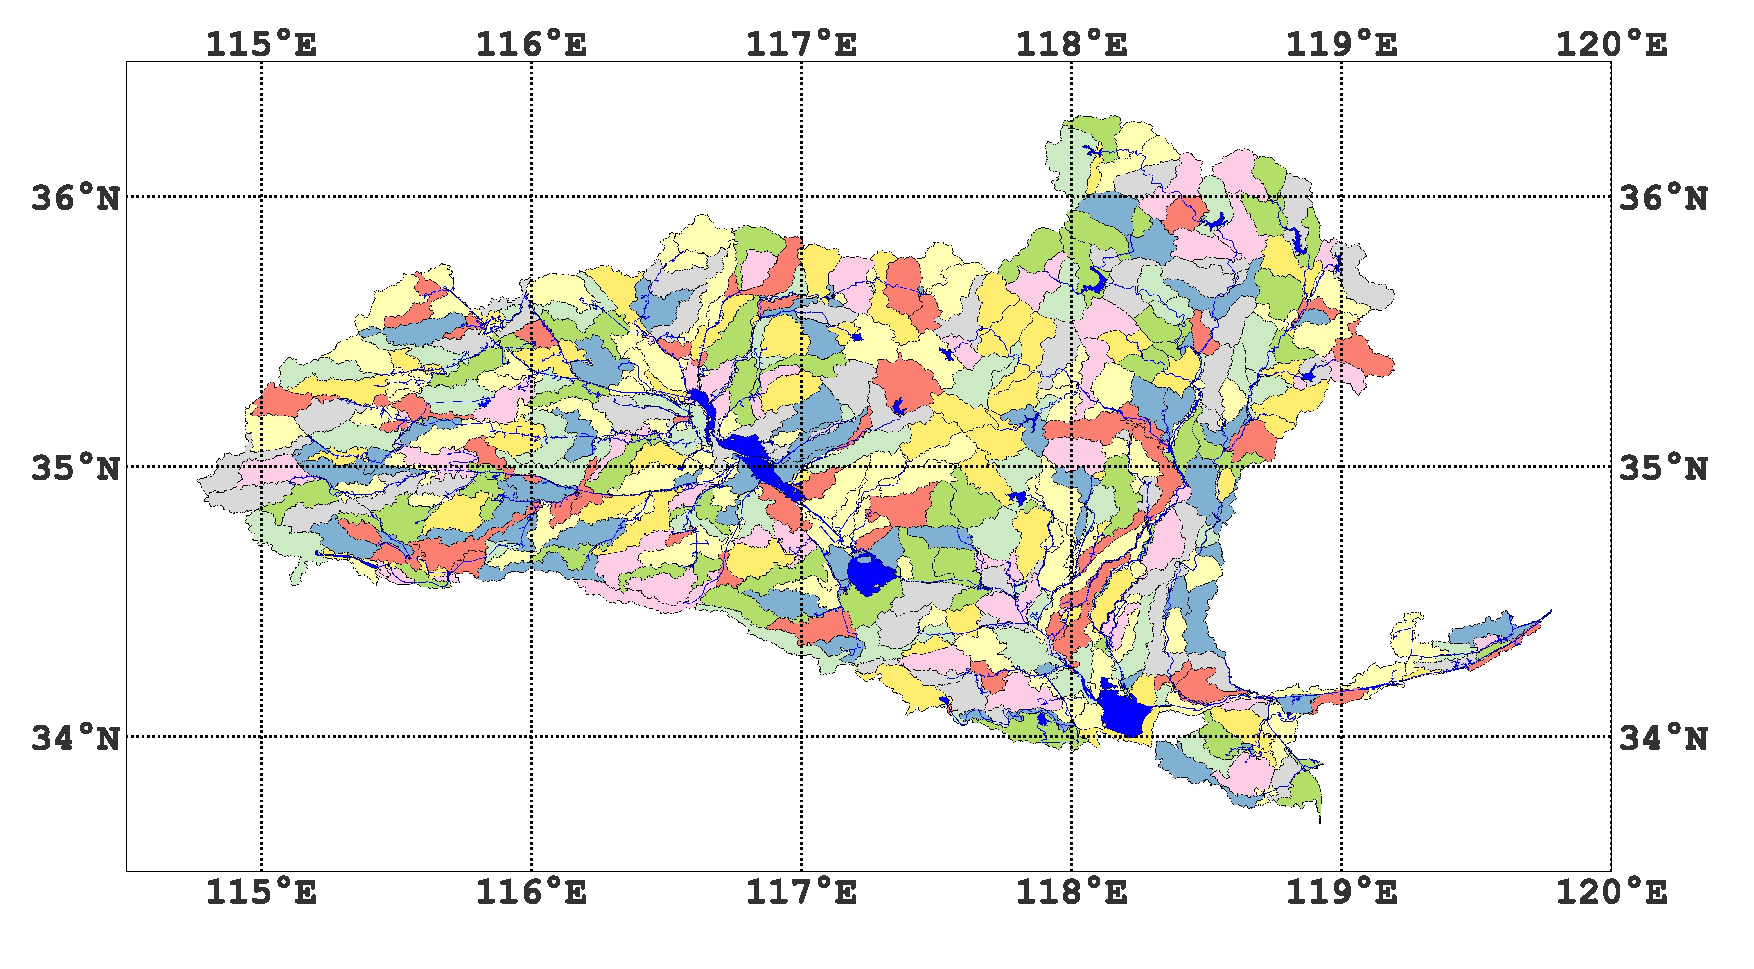
\includegraphics[width=\textwidth]{figures/CatchmentMesh_Huaihe.pdf}
    \caption{基于流域单元网格对淮河流域进行模拟时的流域单元划分图。本实例中,流域单元的面积阈值为250~$\mathrm{km^2}$。图中蓝色部分表示湖泊和河道,其余颜色代表流域单元。}
    \label{fig:fig_huaihe}
\end{figure}

\texttt{define.h}文件的内容为,
\lstinputlisting[language=fortran, basicstyle=\linespread{1.0}\footnotesize\ttfamily, commentstyle=\color{olive}, numbers=left, numberstyle=\tiny, xleftmargin=1.5em,xrightmargin=0em, aboveskip=1em]{examples/catchment/define.h}

Namelist文件的内容为,
\lstinputlisting[language=fortran, basicstyle=\linespread{1.0}\footnotesize\ttfamily, commentstyle=\color{olive}, numbers=left, numberstyle=\tiny, xleftmargin=1.5em,xrightmargin=0em, aboveskip=1em]{examples/catchment/HuaiRiver_Catch_250km2_IGBP_VG.nml}

此实例中,\par
1)区域大致范围通过\texttt{DEF\_domain}进行设定;\par
2)从文件\texttt{DEF\_CatchmentMesh\_data}中的'icatchment2d'变量读入\textbf{描述单元划分的数据};\par
3)文件\texttt{DEF\_ElementNeighbour\_file}中的数据描述了\textbf{侧向流模拟}所需的流域单元及单元之间的参数信息;\par
4)\textbf{并行化}方面,将全球分为5\textdegree$\times$ 5\textdegree 的数据块进行并行模拟(\texttt{DEF\_nx\_blocks}和\texttt{DEF\_ny\_blocks}),每24个进程为一个工作组(\texttt{DEF\_PIO\_groupsize});\par
5)\textbf{地表覆盖类型数据}使用了2005年的数据(\texttt{DEF\_LC\_YEAR});\par
6)\textbf{叶面积指数数据}使用了2005年的月数据(不随年份变化时,叶面积指数数据的年份同\texttt{DEF\_LC\_YEAR}),不随年份变化(\texttt{DEF\_LAI\_CHANGE\_YEARLY});\par
7)使用FIT算法进行\textbf{土壤水热参数升尺度}(\texttt{DEF\_USE\_SOILPAR\_UPS\_FIT});\par
8)使用冷启动的方式对土壤和积雪的状态进行\textbf{初始化}(\texttt{DEF\_USE\_SoilInit}和\texttt{DEF\_\allowbreak USE\allowbreak\_SnowInit});\par
9)使用水体深度动态变化方案(\texttt{DEF\_USE\_Dynamic\_Lake}),其余\textbf{过程参数化方案}均使用模式默认值;\par
10)使用CRUJRA数据作为\textbf{大气驱动}(\texttt{DEF\_forcing\_namelist});\par
11)每月保存一次\textbf{重启动}变量(\texttt{DEF\_WRST\_FREQ});\par
12)\textbf{历史数据的输出},
\begin{itemize}[nosep,leftmargin=4em]
    \item 输出到0.05\textdegree 经纬度网格(\texttt{DEF\_hist\_lon\_res}和\texttt{DEF\_hist\_lon\_res});
    \item 输出变量的日值(\texttt{DEF\_HIST\_FREQ});
    \item 每月的数据保存在一个文件中(\texttt{DEF\_HIST\_groupby});
    \item 输出所有变量(\texttt{DEF\_hist\_vars\_out\_default}).
\end{itemize}\par
13)其他配置使用模式默认值。


\section{实例7:非结构网格单元模拟}

本节配置了一个基于非结构网格单元的实例。实例使用了非结构网格单元,基于地表覆盖类型(IGBP)的植被结构次网格,以及van Genuchten-Mualem土壤水特征曲线模型,并基于MPI进行并行加速。

\texttt{define.h}文件的内容为,
\lstinputlisting[language=fortran, basicstyle=\linespread{1.0}\footnotesize\ttfamily, commentstyle=\color{olive}, numbers=left, numberstyle=\tiny, xleftmargin=1.5em,xrightmargin=0em, aboveskip=1em]{examples/unstructured/define.h}

Namelist文件的内容为,
\lstinputlisting[language=fortran, basicstyle=\linespread{1.0}\footnotesize\ttfamily, commentstyle=\color{olive}, numbers=left, numberstyle=\tiny, xleftmargin=1.5em,xrightmargin=0em, aboveskip=1em]{examples/unstructured/Tibet_unstructured_200km_IGBP_VG.nml}

此实例中,\par
1)区域大致范围通过\texttt{DEF\_domain}进行设定;\par
2)从文件\texttt{DEF\_file\_mesh}中的'elmindex'变量读入\textbf{描述单元划分的数据};\par
3)\textbf{并行化}方面,将全球分为5\textdegree$\times$ 5\textdegree 的数据块进行并行模拟(\texttt{DEF\_nx\_blocks}和\texttt{DEF\_ny\_blocks}),每24个进程为一个工作组(\texttt{DEF\_PIO\_groupsize});\par
5)\textbf{地表覆盖类型数据}使用了2005年的数据(\texttt{DEF\_LC\_YEAR});\par
6)\textbf{叶面积指数数据}使用了2005年的月数据(不随年份变化时,叶面积指数数据的年份同\texttt{DEF\_LC\_YEAR}),不随年份变化(\texttt{DEF\_LAI\_CHANGE\_YEARLY});\par
7)使用FIT算法进行\textbf{土壤水热参数升尺度}(\texttt{DEF\_USE\_SOILPAR\_UPS\_FIT});\par
8)使用热启动的方式对土壤状态进行\textbf{初始化}(\texttt{DEF\_USE\_SoilInit}),初始状态从文件\texttt{DEF\_file\_SoilInit}中读入;\par
9)使用冷启动的方式对积雪的状态进行\textbf{初始化}(\texttt{DEF\_USE\_SnowInit});\par
10)使用ERA5数据作为\textbf{大气驱动}(\texttt{DEF\_forcing\_namelist});\par
11)每月保存一次\textbf{重启动}变量(\texttt{DEF\_WRST\_FREQ});\par
12)\textbf{历史数据的输出},
\begin{itemize}[nosep,leftmargin=4em]
    \item 输出到0.25\textdegree 经纬度网格(\texttt{DEF\_hist\_lon\_res}和\texttt{DEF\_hist\_lon\_res});
    \item 输出变量的月值(\texttt{DEF\_HIST\_FREQ});
    \item 每月的数据保存在一个文件中(\texttt{DEF\_HIST\_groupby});
    \item 输出所有变量(\texttt{DEF\_hist\_vars\_out\_default}).
\end{itemize}\par
13)其他配置使用模式默认值。

\section{辅助工具包}
CoLM2024的辅助工具包包括案例创建、案例复制、案例代码比较、创建配置文件、案例代码更新和拷贝代码6个命令组成,这6个命令互相调用,集成不同的功能脚本。create\_newcase和create\_clone是两个案例创建功能脚本,create\_namelist,create\_script、create\_header和copy\_code是四个基础脚本,用于辅助案例创建的。update\_casecode用于版本控制后的案例代码更新。diff\_casecode用于比较两个案例之间,案例和主代码之间的差异。辅助工具包主要是基于案例的概念进行打造的,每个案例拥有独立案例目录,案例目录下包括独立的代码和配置,也就是说对于案例代码的修改,将不会影响其他案例和主代码,这大大地方便模式开发者对于版本的灵活控制。

\subsection{案例目录的结构}
\subsubsection{案例目录的结构}
执行辅助工具包将自动生成案例目录,案例目录由若干子目录和文件组成,包括代码目录(bld),运行脚本(mksrf.submit, init.submit和case.submit),模拟配置文件(namelist文件),历史文件目录(history$\slash$),重启文件目录(restart$\slash$)和地表数据目录(landdata$\slash$)。其中,代码目录包括源代码目录(bld$\slash$main$\slash$, bld$\slash$mkinidata$\slash$, bld$\slash$mksrfdata$\slash$和bld$\slash$share$\slash$,编译配置文件(bld$\slash$include$\slash$Makeoption)和宏配置文件(bld$\slash$include$\slash$define.h)。历史文件(见章节~\ref{history})、重启文件(见章节~\ref{restart})、地表数据(见章节~\ref{landdata})、namelist文件(见章节~\ref{nml})和宏配置文件(见章节~\ref{define.hux6587ux4ef6})的功能和可选项已在前面章节中详细介绍。代码目录和运行脚本是辅助运行工具包中的新内容。运行脚本用于队列系统的任务提交(如SLURM、LSF和QBS等队列系统),代码目录独立于主目录的代码,可以用于案例的代码修改和初期调试,宏配置文件也在该目录下。修改该目录下的代码或宏文件之后,可以直接编译并单独应用于该案例。

\subsection{辅助工具包的配置}

辅助工具包在移植到新机器使用前需要先编辑机器配置文件和队列系统脚本格式文件,配置并指定数据代码的路径、三个脚本运行需要的核数等机器信息和队列系统脚本格式。机器配置文件包含了新建案例所需的机器信息和数据路径信息(run$\slash$machine.config)见~\ref{table_machineconfig}。

\begin{table}[!htbp]
\caption{机器配置文件变量一览} \label{table_machineconfig}
\centering \renewcommand{\arraystretch}{1.2}
\begin{tabular}{lcp{0.35\textwidth}}
\toprule
\textbf{变量名} & \textbf{示例} & \textbf{说明} \\ \midrule
NProcesses\_mksrf & 672 & mksrf.submit脚本需要的核数 \\
NNodes\_mksrf & 14 & mksrf.submit需要的节点数目 \\
NTasksPerNode\_mksrf & 48 & mksrf.submit单节点核数 \\
Memory\_mksrf & 150G & mksrf.submit运行所申请内存 \\
Walltime\_mksrf & 24:00:00 & mksrf.submit运行所申请时间 \\
Queue\_mksrf & normal & mksrf.submit需要使用的队列 \\
NProcesses\_mkini & 48 &init.submit脚本需要的总核数 \\
NNodes\_mkini & 14 & init.submit需要的节点总数 \\
NTasksPerNode\_mkini & 48 & init.submit单节点核数 \\
Memory\_mkini & 150G & init.submit运行所申请内存 \\
Walltime\_mkini & 24:00:00 & init.submit运行所申请时间 \\
Queue\_mksrf & normal & init.submit需要使用的队列 \\
NProcesses\_case & 48 & case.submit脚本需要的核数 \\
NNodes\_case & 14 & case.submit需要的节点数目 \\
NTasksPerNode\_case & 48 & case.submit单节点核数 \\
Memory\_case & 150G & case.submit运行所申请内存 \\
Walltime\_case & 24:00:00 & case.submit运行所申请时间 \\
Queue\_mksrf & normal & case.submit需要使用的队列 \\
ROOT & \textasciitilde/CoLM/ & 代码个目录路径 \\
RAWDATA & \textasciitilde/rawdata/ & 模型所需的静态原始数据 \\
RUNTIME & \textasciitilde/runtime/ & 模型所需的动态地表数据 \\
MAKEOPTION & Makeoptions & 编译配置 (模板在include/下) \\
FORCINGPATH & \textasciitilde/GSWP3/ &气象驱动数据地址 \\
\bottomrule
\end{tabular}
\end{table}

如须使用队列系统进行任务提交,需要通过编辑队列系统脚本格式文件来配置任务脚本的队列系统头信息格式(run$\slash$batch.config)。

\begin{lstlisting}
##run/batch.config
#------------------------------baiduboat-----------------------------
#!/bin/bash

#BSUB -J <CASENAME>
#BSUB -q <QUEUE>
#BSUB -o colm.o%
#BSUB -e colm.e%
#BSUB -n <NPROCESSES>
#BSUB -R rusage[mem=<MEMORY>]
#BSUB -R span[ptile=<NTASKSPERNODE>]
\end{lstlisting}

其中<CASENAME>是案例名,由案例创建命令create\_newcase收集(章节~\ref{CreateNewcase})。<QUEUE>、<NPROCESSES>、<MEMORY>和<NTASKSPERNODE>分别代表队列名、任务总核数、内存和单节点核数,由机器配置文件(run$\slash$machine.config)收集,见表~\ref{table_machineconfig}。冗余信息需要用\#注释掉。run$\slash$batch.config提供了SLURM、LSF和QBS的模板。

\subsection{案例创建脚本--create\_newcase} \label{CreateNewcase}
create\_newcase 将依照用户指定路径创建新的案例,允许用户按照典型案例配置或自定义案例进行配置的方法创建新的案例。其中包括创建namelist文件,创建运行脚本,创建头文件和代码拷贝,它们分别依赖create\_namelist、create\_script、create\_header和copy\_code四个基础脚本来实现。

创建新案例的方法有两种,典型配置创建案例和自定义配置创建案例。两种方法配置案例成功后,依然可以对案例namelist文件和宏定义\texttt{define.h}文件进行修改,手动修改或添加案例配置。

\subsubsection{典型配置创建案例}

典型配置创建案例语法较简单,适合初级用户快速展开模型运行。

语法:

\begin{lstlisting}
./create_newcase -n {案例运行路径} -c {典型案例配置选项名} [-t {起始年份}] [-e {结束年份}] [-f {气象驱动}]
\end{lstlisting}

案例运行路径为案例的绝对路径或相对路径,要求路径末尾没有"/"符号。典型案例配置选项目前包含5种(见表~\ref{tab:cases_config}),它分别包含了分辨率设置、次网格类型设置、生物地球化学开关和BGC半解析预热开关的设置。


例:
\begin{lstlisting}
./create_newcase -n ~/CoLM202X/cases/50km_PFT -c Global_Grid_50km_PFT_VG
\end{lstlisting}

\begin{table}[!htbp]
\renewcommand{\arraystretch}{1.5}
\centering
\caption{典型案例配置一览}\label{tab:cases_config}
\begin{tabular}{
cccccc} \toprule
\textbf{典型案例配置选项名} & \textbf{分辨率} & \textbf{次网格} & \textbf{BGC} &\textbf{SASU}\\ \midrule
Global\_Grid\_50km\_PFT\_VG & 0.5$\times$0.5 & PFT & 关 &关\\
Global\_Grid\_50km\_USGS\_VG & 0.5$\times$0.5 & USGS & 关 &关\\
Global\_Grid\_50km\_PC\_VG & 0.5$\times$0.5 & PC & 关 & 关\\
Global\_Grid\_2x2\_PFT\_VG\_BGC & 2.5$\times$1.875 & PFT& 开 &关\\
Global\_Grid\_2x2\_PFT\_VG\_BGC-SASU & 2.5$\times$1.875 & PFT& 开 & 开\\
\bottomrule
\end{tabular}
\end{table}

所有典型案例为全球范围配置,如果未开启生物地球化学循环(BGC)时,默认分辨率为全球50km,开启BGC时,默认分辨率为全球2.5$\times$1.875分辨率。次网格包含植被功能型次网格(PFT),植物群落次网格(PC),地表覆盖类型次网格(LC),其中LC按不同数据来源包含了IGBP和USGS两种。SASU开启时,create\_newcase会自动帮助配置半解析加速预热方案(SASU),SASU仅在生物地球化学循环(BGC)开启时有效。

典型案例设置可以同时通过选项-t和-e设置运行起始和结束年份,通过-f选择气象驱动,通过-i设置预热的类型。时间、驱动和预热选项都是可缺失的,如果没有提供,起始和结束年份的默认值分别是1980年和2000年,气象驱动默认选择CRUJRA,预热选项默认关闭。


\subsubsection{自定义配置创建案例}

自定义配置创建案例通过手动配置模型起始时间、气象驱动、预热类型、格点类型(分辨率)、次网格类型、土壤水力参数模型、河道径流模型CaMa开关、生物地球化学模型开关、作物模型开关。其中,作物模型开关在生物地球化学模型开启时才生效;格点类型(分辨率)、次网格类型、土壤水力参数模型、河道径流模型CaMa开关、生物地球化学模型开关、作物模型开关在没有出现典型配置选项“-c”时才生效。

语法:
\begin{lstlisting}
./create_newcase -n {案例运行路径} [ -t {开始年份} ] [ -e {结束年份}] [ -f {气象驱动}] [ -g {格点类型} ] [ -s {次网格方案}] [ -m {土壤水力参数模型}] [ -r ] [-b [-p] [-i {预热方案}] ]
\end{lstlisting}

案例运行路径为案例的绝对路径或相对路径,要求路径末尾没有"/"符号。自定义案例配置的详细配置见表~\ref{tab:custom_option}。所有自定义选项均为可缺失选项,缺省值见表~\ref{tab:custom_option}。

例:
\begin{lstlisting}
./create_newcase -n ~/CoLM202X/cases/50km_PFT -t 1980 -e 2000  -g grid_g144x96 -s PFT -m vg -b -i sasund
\end{lstlisting}

\begin{table}[!htbp]
\renewcommand{\arraystretch}{1.5}
\centering
\caption{自定义案例配置选项一览}\label{tab:custom_option}
\begin{tabular}{
cccccc} \toprule
\textbf{配置选项内容} & \textbf{配置选项} & \textbf{缺省值} & \textbf{备选值} & \textbf{有效条件}\\ \midrule
开始年份 & -t & 1980 & 任意整数 & 始终有效\\
结束年份 & -e & 2000 & 任意整数 & 始终有效\\
气象驱动 & -f & CRUJRA & CRUJRA; GSWP3  & 始终有效\\
格点类型 & -g & $\mathrm{grid}\_\mathrm{g}720\mathrm{x}360$ & 无& 无 -c\\
次网格方案 & -s & PFT & USGS; IGBP; PFT; PC & 无 -c\\
土壤水力模型 & -m & vg & vg; cb& 无 -c\\
Cama模型 & -r & 关 & 无& 无 -c\\
BGC模型 & -b & 关 & 无& 无 -c\\
作物模型 & -p & 关 & 无& 无 -c有 -b\\
预热方案 & -i & none & none; nd; sasund& 无 -c有 -b\\
\bottomrule
\end{tabular}
\end{table}

自定义案例配置选项按照有效条件可以任意组合,对新建案例进行配置,配置完成后,仍然可以通过文本编辑修改\texttt{define.h}, namelist以及三个任务提交脚本进行修改。

\subsection{案例复制脚本--create\_clone}

在方案比较实验中,经常需要运行两个配置相似的案例。使用案例复制命令create\_clone可以大大提高工作效率,并且降低配置出错的概率。

语法:
\begin{lstlisting}
./create_clone -s {待拷贝案例路径} -d {新案例路径}
\end{lstlisting}

例:
\begin{lstlisting}
./create_clone -s ~/CoLM202X/cases/50km_PFT -d ~/CoLM202X/cases/50km_PFT-new
\end{lstlisting}

待拷贝案例路径和新案例路径都要求路径末尾没有"/"符号。create\_clone语句将拷贝原案例的代码(bld目录)、运行脚本和namelist文件,并且识别案例名,对脚本和namelist中的案例名进行替换。

\subsection{案例的编译和运行}
\subsubsection{案例的编译}
对于案例代码的编译需要进入bld目录,并运行make命令。make前要确认编译配置文件(bld$\slash$include$\slash$Makeoption)的设置是否正确,包括netcfd库,Fortran编译器的选项和路径等(见章节~\ref{comprun})。

\subsubsection{案例目录的运行}
对于典型案例我们提供了适用于队列系统任务提交的三个脚本:地表数据制作任务提交脚本mksrf.submit,初始化任务提交脚本init.submit和模型运行任务提交脚本case.submit,他们分别对应章节~\ref{runcolm}中提到的三个colm运行步骤:地表数据制作、初始场数据制作和主程序运行。运行前需要检查队列系统所需要核数的设置是否和运行mpirun中要求的核数一致,其他内存和队列等配置是否符合服务器的要求。

\subsection{辅助工具包高级功能}

\subsubsection{案例代码的比较--diff\_casecode.bash}

在代码开发过程中,需要比较两个代码的差异,案例代码比较脚本可以帮助比较案例代码之间和案例代码与主代码的区别。

语法:

\begin{lstlisting}
./diff_casecode.bash {待比较案例1路径} [ {待比较案例2路径} ]
\end{lstlisting}

例:
\begin{lstlisting}
./diff_casecode.bash ~/CoLM202X/cases/50km_PFT ~/CoLM202X/cases/50km_PFT-new1
或
./diff_casecode.bash  ~/CoLM202X/cases/50km_PFT
\end{lstlisting}

diff\_casecode.bash后可接两个参数或一个参数,参数指明案例路径,要求路径末尾没有"/"符号。当脚本命令后接两个参数并指定两个案例路径时,脚本将比较两个案例代码之间每行的差异。当脚本命令后接一个参数并制定一个案例路径时,脚本将比较该案例代码和主代码之间的差异,主代码路径需要通过编辑diff\_casecode.bash文件“ROOT=”行内容来指定。

\subsubsection{案例namelist文件的创建--create\_namelist}

模式运行的namelist文件可以通过create\_namelist脚本来创建。create\_namelist根据输入的开始结束年份、气象驱动、原始地表数据路径、运行数据路径、陆海分布数据、BGC预热方案和运行区域信息写入namelist文件。create\_namelist脚本所有选项一览表见表~\ref{tab:createnml_option}。

语法:
\begin{lstlisting}
./create_namelist {案例路径} {案例名} [-t {开始年份} ] [ -e {结束年份}] [ -f {气象驱动}] [ -d {原始地表数据路径}] [ -r {运行时数据路径}] [ -a {格点纬向分辨率} ] [ -o {格点经向分辨率} ] [ -S {区域南边界纬度} ] [ -N {区域北边界纬度} ] [ -E {区域东边界经度} ] [ -W {区域西边界经度} ] [ -i {BGC预热方案} ]
\end{lstlisting}

例:
\begin{lstlisting}
./create_namelist -p ~/CoLM202X/cases/ -n 50km_PFT -a 0.5 -o 0.5
\end{lstlisting}

\begin{table}[!htbp]
\renewcommand{\arraystretch}{1.5}
\centering
\caption{create\_namelist配置选项一览}\label{tab:createnml_option}
\begin{tabular}{
cccccc} \toprule
\textbf{配置选项内容} & \textbf{配置选项} & \textbf{缺省值} & \textbf{备选值} & \textbf{有效条件}\\ \midrule
案例路径 & -p & 不可缺省 & 任意路径 & 始终有效 \\
案例名  & -n & 不可缺省 & 任意字符串 & 始终有效 \\
开始年份 & -t & 1980 & 任意整数 & 始终有效\\
结束年份 & -e & 2000 & 任意整数 & 始终有效\\
气象驱动 & -f & CRUJRA & CRUJRA; GSWP3  & 始终有效\\
原始地表数据路径 & -d & 无 & 任意路径 & 始终有效\\
运行数据路径 & -r & 无 & 任意路径 & 始终有效\\
经向分辨率 & -a & 0.5 & 任意数值 & 始终有效\\
纬向分辨率 & -o & 0.5 & 任意数值 & 始终有效\\
海陆分布数据路径 & -l & 无 & 任意路径 & 始终有效\\
区域南边界纬度 & -S & -90 & -90.0\textasciitilde90.0 小于北边界纬度 & 始终有效\\
区域北边界纬度 & -N & 90 & -90.0\textasciitilde90.0 大于南边界纬度 & 始终有效\\
区域西边界经度 & -S & -180 & -180.0\textasciitilde180.0 小于东边界经度 & 始终有效\\
区域东边界经度 & -N & 180 & -180.0\textasciitilde180.0 大于西边界经度 & 始终有效\\
BGC预热开关 & -i &none & none; nd; sasund& 始终有效 \\
\bottomrule
\end{tabular}
\end{table}

\subsubsection{案例脚本的创建--create\_script}

create\_script可以帮助用户生成可用于队列系统的三个任务脚本(mksrf.submit, init.submit和case.submit)。每个任务脚本根据batch.config和machine.config的内容来完成头信息的配置,它指定节点数目、CPU数目、内存使用和运行时间长度。create\_namelist脚本所有选项一览表见表~\ref{tab:createscript_option}。

create\_script根据BGC预热开关的设置(-i选项),为case.submit配置三种不同的预热方式:1) none, 2) nd, 3) sausund。BGC预热要求用脚本来控制单年驱动循环,1) none方式不包含BGC预热,可以用于非循环的模拟,为默认方案;2) nd方式为一年驱动循环的预热方式,case.submit中包含循环末尾对重启文件的重命名(时间戳的重命名),默认完成100次循环,可生脚本后通过手动编辑case.submit进行修改。3) sasund方式同为1年驱动循环的预热,case.submit中包含循环末尾对重启文件的重命名(时间戳重命名),默认完成130次循环,但前100次为半解析加速预热,后三十次为普通预热方式,类同于nd方式。

语法
\begin{lstlisting}
./create_scripts -p {案例路径} -t {开始年份} -e {结束年份} -f {batch配置文件路径} -c {机器配置文件路径} -i {BGC预热方案}
\end{lstlisting}

例:
\begin{lstlisting}
./create_scripts -p ~/CoLM202X/cases/50km_PFT -t 1850 -e 1850 -f ~/CoLM202X/run/batch.config -c ~/CoLM202X/run/machine.config -i nd
\end{lstlisting}

\begin{table}[!htbp]
\renewcommand{\arraystretch}{1.5}
\centering
\caption{create\_script配置选项一览}\label{tab:createscript_option}
\begin{tabular}{
cccccc} \toprule
\textbf{配置选项内容} & \textbf{配置选项} & \textbf{缺省值} & \textbf{备选值} & \textbf{有效条件}\\ \midrule
案例路径名 & -p & 不可缺省 & 任意路径 & 始终有效 \\
开始年份 & -t & 不可缺省 & 任意整数 & 始终有效\\
结束年份 & -e & 不可缺省 & 任意整数 & 始终有效\\
batch配置文件路径 & -f & 不可缺省 & 任意路径 & 始终有效 \\
机器配置文件路径 & -f & 不可缺省 & 任意路径 & 始终有效 \\
BGC预热开关 & -i &none & none; nd; sasund& 始终有效 \\
\bottomrule
\end{tabular}
\end{table}

\subsubsection{案例代码更新--update\_casecode}

随着代码的发展,本地仓库会通过github进行更新。案例代码常常需要随着本地仓库代码的更新而更新。运用案例代码更新脚本可以帮助实现案例代码的更新。但需注意,案例代码更新脚本仅仅实现拷贝覆盖代码的功能,尚无法实现代码合并(merge)的功能。因此,更新代码前须妥善处理案例代码已更新的部分。注意:在使用前,需要编辑update\_casecode中的ROOT变量,定位本地仓库代码。

语法:
\begin{lstlisting}
./update_casecode {待更新的案例路径}
\end{lstlisting}
另外,确保待更新的案例路径后没有"/"。

例:
\begin{lstlisting}
./update_casecode ~/CoLM202X/cases/50km_PFT
\end{lstlisting}


\subsubsection{案例代码复制--copy\_code}
copy\_code将原案例或本地仓库代码拷贝到新案例代码路径,是案例复制脚本(create\_clone)和案例代码更新脚本(update\_casecode)的一部分。相比create\_clone,copy\_code的差异在于它仅拷贝代码不操作namelist和任务脚本文件。注意:案例代码路径需要给到案例的bld目录地址,本地仓库代码路径给到本地仓库地址即可。

语法:
\begin{lstlisting}
./copy_code -s {待复制代码路径} -d {目标代码路径}
\end{lstlisting}

例:
\begin{lstlisting}
./copy_code -s ~/CoLM202X/cases/50km_PFT/bld -d ~/CoLM202X/cases/50km_PFT-new1/bld
或
./copy_code -s ~/CoLM202X -d ~/CoLM202X/cases/50km_PFT-new1/bld
\end{lstlisting}
第二个例子等同于用update\_casecode更新案例50km\_PFT-new1

\clearpage
